\documentclass[11pt,journal,onecolumn]{IEEEtran}
\usepackage{amsmath,amssymb,bm,amsthm,amstext}
\usepackage{enumerate,longtable,tikz,subfigure,float}
\usepackage{cite,color}
\usetikzlibrary{decorations.pathreplacing}

\begin{document}

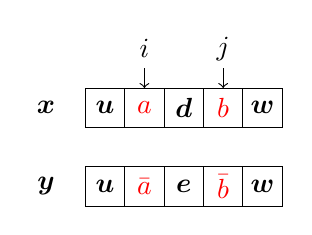
\begin{tikzpicture}
\draw (0,0) rectangle (0.5,0.5);
\draw (0.5,0) rectangle (1,0.5);
\draw (1,0) rectangle (1.5,0.5);
\draw (1.5,0) rectangle (2,0.5);
\draw (2,0) rectangle (2.5,0.5);
\path (0.25,0.25)node{$\bm{u}$}
      (0.75,0.25)node{\textcolor{red}{$a$}}
      (1.25,0.25)node{$\bm{d}$}
      (1.75,0.25)node{\textcolor{red}{$b$}}
      (2.25,0.25)node{$\bm{w}$}
      (-0.5,0.25)node{$\bm{x}$};
\draw (0,-1) rectangle (0.5,-0.5);
\draw (0.5,-1) rectangle (1,-0.5);
\draw (1,-1) rectangle (1.5,-0.5);
\draw (1.5,-1) rectangle (2,-0.5);
\draw (2,-1) rectangle (2.5,-0.5);
\path (0.25,-0.75)node{$\bm{u}$}
      (0.75,-0.75)node{\textcolor{red}{$\bar{a}$}}
      (1.25,-0.75)node{$\bm{e}$}
      (1.75,-0.75)node{\textcolor{red}{$\bar{b}$}}
      (2.25,-0.75)node{$\bm{w}$}
      (-0.5,-0.75)node{$\bm{y}$};
\draw[->](0.75,0.75)--(0.75,0.5);
\draw[->](1.75,0.75)--(1.75,0.5);
\draw (0.75,1)node{$i$};
\draw (1.75,1)node{$j$};
\end{tikzpicture}

\end{document}